\Section{Discussion}
\label{sec:discussion}

  In this section, we discuss our findings and prospects for future work.

\SubSection{Extensibility}

  One of our goals was to provide fully bi-directional transformations
between textually-written code and graphical tiles.  We succeeded in doing this.  However,
we feel that our
implementation is not as deeply extensible as it should be,
for we can neither view nor modify the
semantics and syntax of the language itself.

  We had attempted to define a method called {\tt eval()} in
JavaScript for each kind of parse node; i.e, we tried to provide a
meta-circular implementation of JavaScript which
could be viewed and modified in the same system.  However, a
meta-circular definition has to have a fixed point, and we realized
that the fixed point cannot be so {\em deep}; a function definition
requires functions defined, a function call uses many function calls,
getters and setters get and set values from objects, and {\tt if}
requires a {\tt if} statement.  These facilities cannot be written in
the user-level language.  In the other words, they have to be
``primitives'' and the user cannot modify them, for example, using tiles.

  In this sense, we contend that the macro system provides better
separation between the base language and the language that the
end-user works with.  For example, consider the {\tt @if} macro.  The user can
still change the look of its associated tile, and even change its semantics.
From the user's point
of view, this is a very powerful concept even though he can neither
change nor even see the definition of {\tt if} in the base language,

  We would like to revisit this issue in the future and try to
define a language with a smaller core.

\SubSection{The Choice of Base Language}

The choices of base language and end-user language have interesting
trade-offs.  Having a mainstream syntax helps to lower the
learning curve in a practical sense, but from the standpoint of
making text and tiles isomorphic, it can be problematical.

For instance, we would like to provide a model of the grammar that advanced end-users
can access and understand.  One of the authors made a kind of a visual
grammar editor called LanguageGame~\cite{ty03languagegame}.  We plan
to experiment with an end-user grammar editor along the line of
LanguageGame.

Had we decided to use a language with uniform syntax, like LISP or Scheme,
as our base language, it would be fairly easy for end-users to understand the
grammar, because it would be so simple.
Javascript syntax has a much more complex grammar, and will certainly make
the addition of extensible syntax to our system more difficult on the end-user.

\SubSection{The Type System}
  One of the biggest advantages of tile scripting is that it can be
made type-safe without any additional complexity.
The drag-and-drop interface can be made so that only
type-conforming tiles may be combined, and the resulting script
doesn't produce any run time errors.

  TileScript does not currently have any type-checking mechanisms.
Since TileScript allows textual coding and conversion to tiles, developing a
reasonable type system will be an interesting challenge.

\SubSection{Formatting Textual Code}

  In the current implementation, parse tree nodes do not carry any
information about the formatting of their corresponding textual code.  Consider what happens when the user writes
some code textually, converts it to tiles, and then makes some very small
modification.  If he converts the tiles back to textual code, all
formatting information such as indentation and line breaks will be lost.
In order to minimize such nasty surprises, TileScript parse tree nodes should contain as much formatting
information as possible (these should be stored as properties), and the different conversions
take them into account.

\SubSection{Structure of Tiles}
  In our current implementation, the visual appearance of a tile
script follows the structure of the parse tree.  This is fine in most of the
cases, but can be cumbersome for a chain of arithmetic operators.  For
example, if the user thinks about an expression:
\begin{center}
{\tt sum = a + b + c + d + e}
\end{center}
he does not need to think about operator precedence; it is better
to simply think of the above expression as the ``sum of five values''.
However, the in the tile representation, the user is inevitably forced
to look at nested expressions as shown in Figure~\ref{fig:nested
tiles}.  A sophisticated tile scripting environment should allow the
user to edit such expressions in less rigid ways.

\begin{figure}[tp]
\centering
\scalebox{0.5}{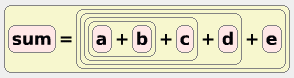
\includegraphics{sum.eps}}
\caption{A nested tree from a flat expression.}
\label{fig:nested tiles}
\end{figure}

